\chapter{Avance del objetivo específico 1}

\section{Caracterización de HAM10000}

HAM10000 contiene 10.015 imágenes dermatoscópicas distribuidas en siete clases \parencite{tschandl2018ham10000}. La clase \texttt{nv} concentra la mayoría de las imágenes. \texttt{akiec} agrupa queratosis actínica y carcinoma intraepidérmico; no representa una clase independiente de carcinoma escamocelular invasor. La diferencia entre distribución del conjunto y perfil epidemiológico regional limita la interpretación de resultados como representatividad de Santander.

\begin{figure}[htbp]
\centering
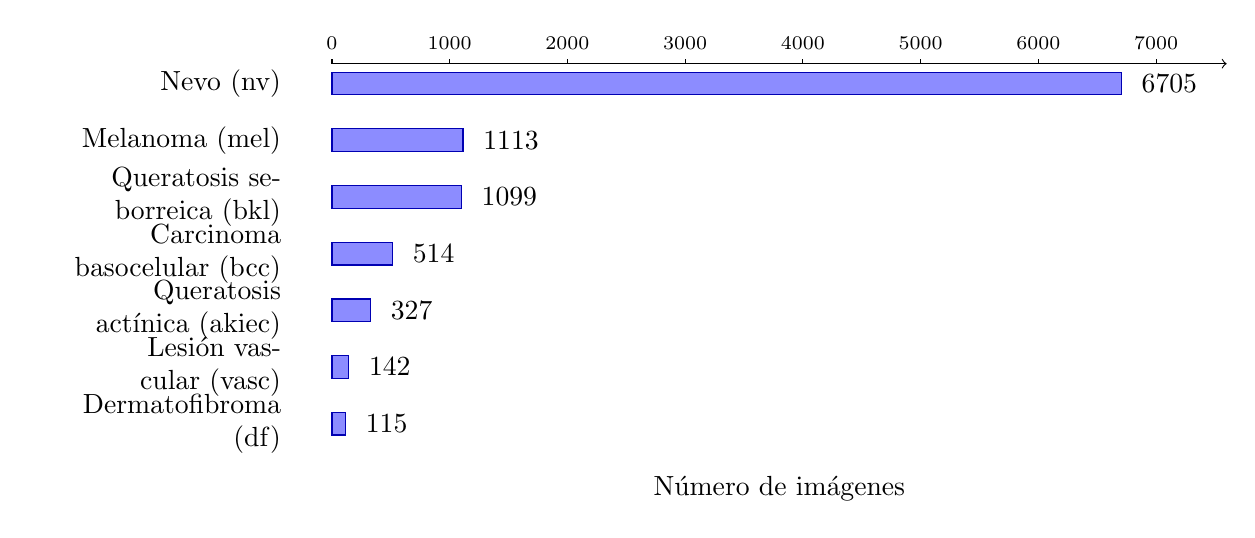
\begin{tikzpicture}[x=0.0015cm,y=0.72cm]
    \draw[->] (0,0) -- (7600,0);
    \foreach \tick in {0,1000,...,7000} {
        \draw (\tick,0) -- (\tick,0.08) node[above] {\scriptsize \tick};
    }
    \foreach \y/\clase/\valor in {
        0/Nevo\ (nv)/6705,
        1/Melanoma\ (mel)/1113,
        2/Queratosis\ seborreica\ (bkl)/1099,
        3/Carcinoma\ basocelular\ (bcc)/514,
        4/Queratosis\ actínica\ (akiec)/327,
        5/Lesión\ vascular\ (vasc)/142,
        6/Dermatofibroma\ (df)/115
    } {
        \draw[fill=blue!45,draw=blue!70!black] (0,-\y-0.55) rectangle (\valor,-\y-0.15);
        \node[anchor=east,align=right,text width=3.1cm] at (-350,-\y-0.35) {\clase};
        \node[anchor=west] at (\valor+90,-\y-0.35) {\valor};
    }
    \node[below] at (3800,-7.1) {Número de imágenes};
\end{tikzpicture}
\caption{Distribución de clases en HAM10000.}
\label{fig:ham10000-clases}
\end{figure}
\noindent\textit{Nota.} Conteos según Tschandl et al. (2018). La distribución es descriptiva y no representa la prevalencia poblacional de Santander.

\section{Cobertura regional y límites del corpus}

La caracterización vincula los conjuntos públicos con las patologías regionales sin asumir cobertura completa. HAM10000 permite estudiar las siete categorías dermatoscópicas enumeradas, pero no incluye una clase separada de SCC invasor ni patologías como leishmaniasis. El estudio local de Uribe et al. documenta carcinoma basocelular en Bucaramanga, pero no basta para inferir conteos acumulados de todas las neoplasias del HIC o mortalidad por melanoma \parencite{uribe2018bccbucaramanga}.

\begin{itemize}
    \item \textbf{ISIC2019/ISIC2020:} fuentes que aparecen en el conjunto no etiquetado según los manifiestos de las corridas; falta publicar en este capítulo el inventario de identificadores y sus hashes.
    \item \textbf{BCN20000:} no se presenta como validación independiente si hay solapamiento con ISIC2019.
    \item \textbf{CO2Wounds-V2:} excluido del núcleo clasificatorio porque contiene heridas crónicas y no imágenes dermatoscópicas de lesiones comparables.
    \item \textbf{PAD-UFES-20:} reservado para evaluación externa de dominio, sin entrenamiento ni ajuste del modelo.
\end{itemize}

\section{Evidencia regional pendiente de consolidación}

\noindent\textbf{[Pendiente de fuente institucional primaria:]} incorporar la tabla de patologías regionales con fuente, año, población, definición de caso y alcance geográfico. Verificar las cifras atribuidas al HIC (3.060 casos y mortalidad por melanoma) antes de incluirlas. La cifra nacional de 11.064 corresponde a casos atendidos de melanoma cutáneo hasta el 31 de diciembre de 2024 y la Cuenta de Alto Costo la reporta como preliminar \parencite{cuentaaltocosto2025melanoma}.

\section{Estado del objetivo}

La identificación y el análisis exploratorio de conjuntos constituyen evidencia de avance del objetivo 1. Antes de declarar el objetivo cerrado, documentar los criterios de selección y exclusión, licencias, grupos de lesión, hashes de las particiones y correspondencia entre cada afirmación epidemiológica y su fuente primaria.
